\documentclass[main]{subfiles}

\begin{document}
    \begin{Utv}
        \[\abs{n_u \times n_v} = \frac{\abs{LN - M^2}}{\sqrt{EG - F^2}}\]
        \[\frac{\abs{n_u \times n_v}}{\abs{r_u \times r_v}} = K = \frac{LN - M^2}{EG - F^2}\]
    \end{Utv}

    \begin{Definition}
        \[(r_u;\ r_v;\ n) \text{ --- базис}\]
        \[r_u \perp n\]
        \[r_v \perp n\]
        \[\abs{n} = 1\]
        \[\abs{r_u} = \sqrt{E}\]
        \[\abs{r_v} = \sqrt{G}\]
        \[\cos \angle(r_u, r_v) = \frac{F}{\sqrt{EG}}\]
    \end{Definition}

    \begin{Reminder}
        \[|r_u \times r_v| = \sqrt{EG - F^2}\]
    \end{Reminder}

    \begin{Proof}
        \[|n_u \times n_v| = \Big| \Br{\frac{MF - LG}{EG - F^2} r_u + \frac{LF - ME}{EG - F^2} r_v} \times \]
        \[\times \Br{\frac{NF - MG}{EG - F^2}r_u + \frac{MF - NE}{EG - F^2}r_v}\Big| =\]
        \[= \frac{1}{(EG - F)^2} |(MF - LG)(NF - MG)\us{=0}{(r_u \times r_u)} + (MF - LG)(MF - NE)(r_u \times r_v) +\]
        \[+ (LF - ME)(NF - MG)(r_v \times r_u) + (LF - ME)(MF - NE)\us{=0}{(r_v \times r_v)}|\]
        \[= \frac{1}{(EG - F)^{\frac{3}{2}}} \abs{(MF - LG)(MF - NE) - (LF - ME)(NF - MG)}} =\]
        \[= \frac{1}{(EG - F^2)^{\frac{3}{2}}} |M^2 F^2 - \cancel{LMFG} - \cancel{MNEF} + LNEG -\]
        \[ - LNF^2 + \cancel{LMFG} + \cancel{MNEF} - M^2 EG}| =\]
        \[= \frac{1}{(EG - F^2)^{\frac{3}{2}}} \abs{(LN - M^2)(EF - F^2)} = \frac{|LN - M^2|}{\sqrt{EG - F^2}}\]
    \end{Proof}

    \subsection{Символы Кристоффеля}
    \begin{theorem}
        $\Gamma_{ij}^k$ относ. к внутренней геометрии
    \end{theorem}

    \begin{Proof}
        \[r_{uu} = \Gamma_{11}^1 r_u + \Gamma_{11}^2 r_v + Ln \q | \cdot r_u \q | \cdot r_v\]
        \[r_{uu} r_u = \Gamma_{11}^1 E + \Gamma_{11}^2 F\]
        \[r_{uu} r_v = \Gamma_{11}^1 F + \Gamma_{11}^2 G\]
        \[E_u = (r_u r_u)'_u = 2 r_{uu} r_v\]
        \[F_u = (r_u r_v)_u = r_{uu} r_v + r_u r_{uv}\]
        \[E_v = (r_u r_u)_v = 2 r_{uv} r_u\]
        \[F_u - \frac{1}{2}E_u = r_{uu} r_u = \Gamma_{11}^1 E + \Gamma_{11}^2 F\]

        Заметим, что система невырожденная, поэтому символы Кристофеля выражаются и зависят только от первой формы.\\

        Аналогично остальные $\Gamma_{ij}^k$

        Проверим некоторые:
        \[\begin{cases}
            \Gamma_{12}^1 E + \Gamma_{12}^2 F = r_{uv} r_u = \frac{1}{2} E_v\\
            \Gamma_{12}^1 F + \Gamma_{12}^2 G = r_{uv} r_v = \frac{1}{2} G_u
        \end{cases}\]
    \end{Proof}

    \subsection{Геодезическая кривизна}
    \begin{Definition}
        \[k_{n} = \pr_{\ol{n}} \vec{k} \text{ --- \ul{нормальная кривизна}}\]
    \end{Definition}
    \begin{figure}[H]
        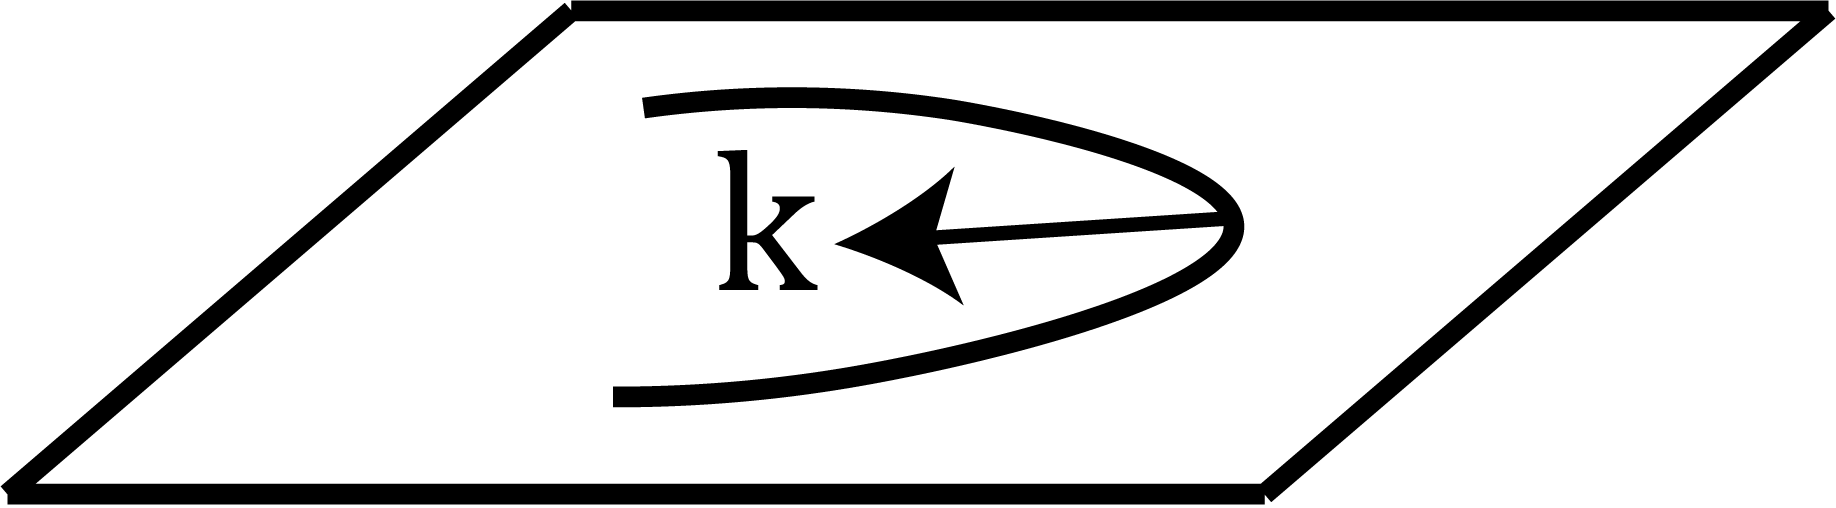
\includegraphics[width=5cm]{pics/11_1.png}
        \centering
    \end{figure}

    \begin{Definition}
        \[k_g := |\pr_{\text{кас. пл.}} \vec{k}| \text{ --- \ul{геодезическая кривизна}}\]
    \end{Definition}
    \begin{figure}[H]
        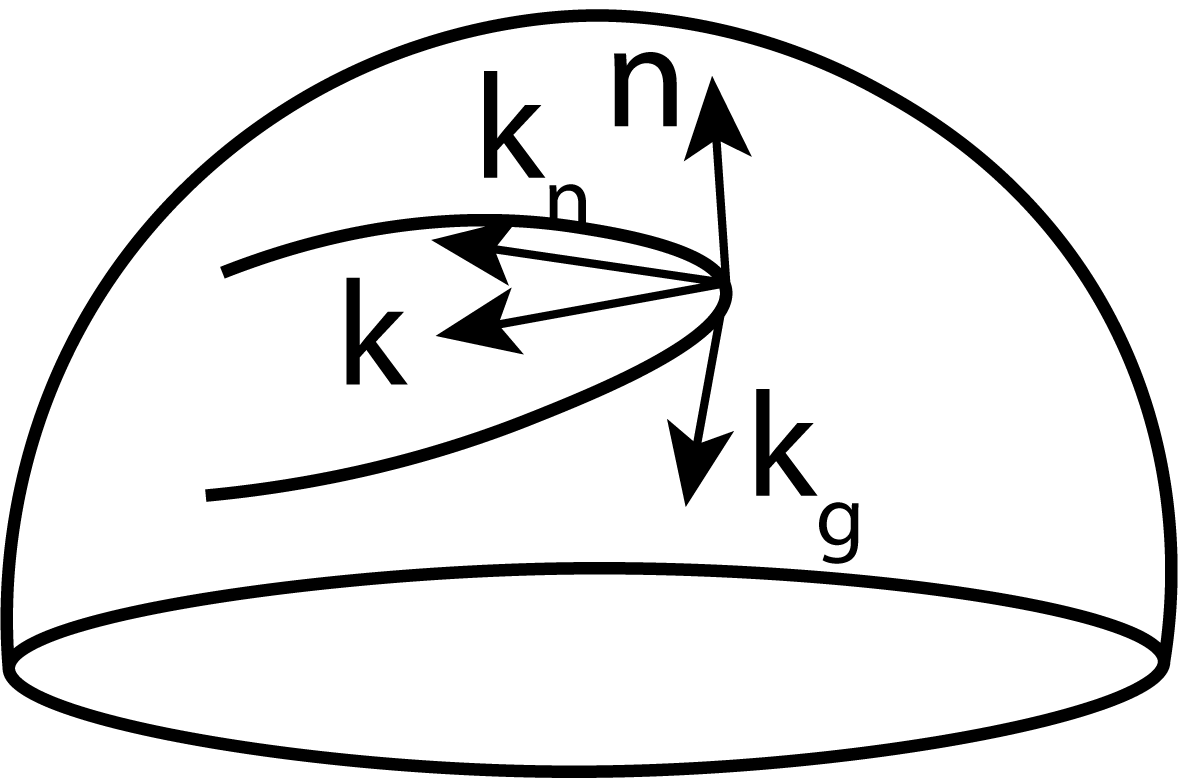
\includegraphics[width=4.5cm]{pics/11_2.png}
        \centering
    \end{figure}

    \begin{Property}
        \[k^2 = k_n^2 + k_g^2\]
    \end{Property}

    \begin{theorem}
        $k_g$ относ. к внутренней геометрии
    \end{theorem}

    \begin{proof}
        Будем рассматривать натуральную параметризацию $(u(s),\ v(s))$
        \[\vec{k} = \frac{d^2}{d s^2} \ol{r}(u(s),\ v(s))\]
        \[\frac{d}{ds} \ol{r} (u(s),\ v(s)) = r_u u' + r_v v'\]
        \[\vec{k} = \frac{d^2}{ds} r(u(s),\ v(s)) = r_{uu} u'^2 + 2 r_{uv} u' v' + r_{vv} v'^2 + r_u u'' + r_v v''\]
        \[\vec{k}_n = (L u'^2 + 2 M u' v' + N v'^2) \cdot \vec{n} \text{ --- знаем}\]
        \[\vec{k} = \ul{(\Gamma_{11}^1 r_u + \Gamma_{11}^2 r_v) u'^2 + 2 (\Gamma_{12}' r_u + \Gamma_{12}^2 r_v) u' v' + (\Gamma_{22}' r_u + \Gamma_{22}^2 r_v) v'^2 +}\] %заменить \ul на волнистое подчеркивание
        \[\ul{r_u u'' + r_v v''} + \vec{n}(Lu'^2 + 2Mu'v' + Nv'^2)\]
        \[k_g = \ul{\q}\]
        \[\ul{\q} = A r_u + B_{r_v}\]
        $A,\ B$ --- только от \RNUmb{1} формы
        \[|k_g| = \sqrt{A^2 E + 2ABF + B^2 G}\]
        \[\vec{k}_g = A \vec{r}_u + B \vec{r}_v\]
        \[|k_g| = \sqrt{(A r_u + B r_v)(A r_v + B r_v)} = \sqrt{A^2 \ub{E}{r_u r_u} + 2 AB \ub{F}{r_u r_v} + B\ub{G}{r_v r_v}}\]
    \end{proof}

    \subsection{Вычисление геодезической кривизны}
    \begin{definition}
        \ul{Геодезической} называется линия, у которой $k_g = 0$
    \end{definition}

    \begin{Utv}[формула]
        \[k_g = \frac{(\varphi'',\ \varphi',\ n)}{|\varphi'|^3} \qq \varphi(t) = r(u(t),\ v(t))\]
    \end{Utv}

    \begin{Proof}
        \[k = \frac{|\varphi'' \times \varphi'|}{|\varphi'|^3}\]
        Разложим $\varphi''$ по двум компонентам:
        \[\varphi_1'' \in \text{кас. пл-ти, } \varphi_2'' \in \text{норм. пл-ти}\]
        \[\varphi_1'' = \pr_{\alpha} \varphi'' \q \varphi_2 = \pr_n \varphi''\]
        \begin{figure}[H]
            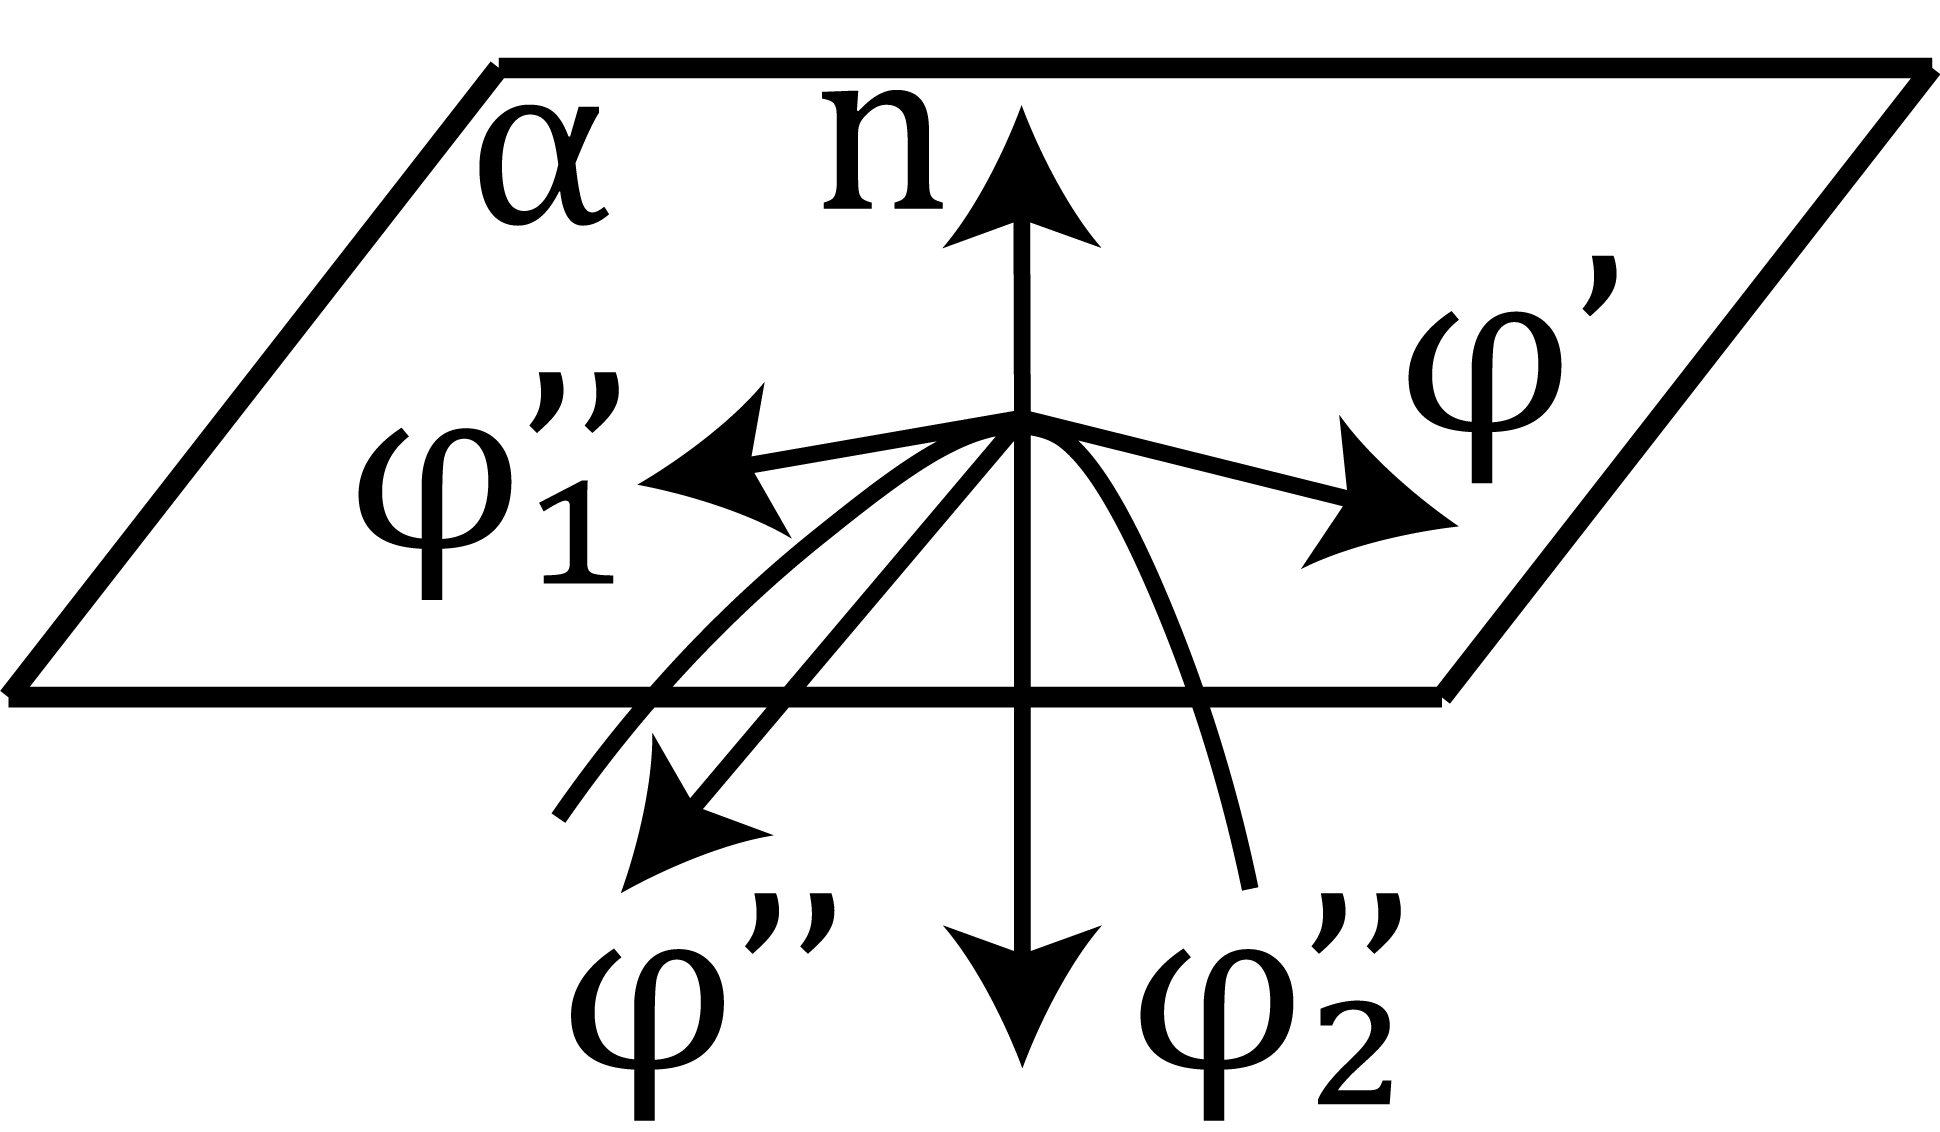
\includegraphics[width=5cm]{pics/11_3.png}
            \centering
        \end{figure}
        \[\varphi'' \times \varphi' = (\varphi''_1 + \varphi''_2) \times \varphi' = \ub{||n}{\varphi''_1 \times \varphi'} + \ub{\bot n}{\varphi''_2 \times \varphi'}\]
    \end{Proof}

    \begin{utv}
        Следующие определения геодезической линии эквивалентны:
        \begin{enumerate}
          \item $k_g = 0$
          \item Соприкасающая пл-ть содержит $\ol{n}$
          \item Спрямляющая пл-ть $=$ кас. пл-ть к пов-ти
          \item $k = k_n$
          \item Кривая с наим. кривизной
          \item (б/д в одну сторону) Локально кратчайшая кривая
          %рисунок, поясняющий последний пункт. Шар со всевозможными сечениями, проходящими через центр сферы
          %1. если есть две точки (A и B), то кратчайшая кривая - геодезическая (если она существует)
          %2. если (A и B) лежат в мал. пов-ти... строго определения я вам не дам (с) Солынин
          %нарисовали рисунок цилиндра
          \begin{figure}[H]
              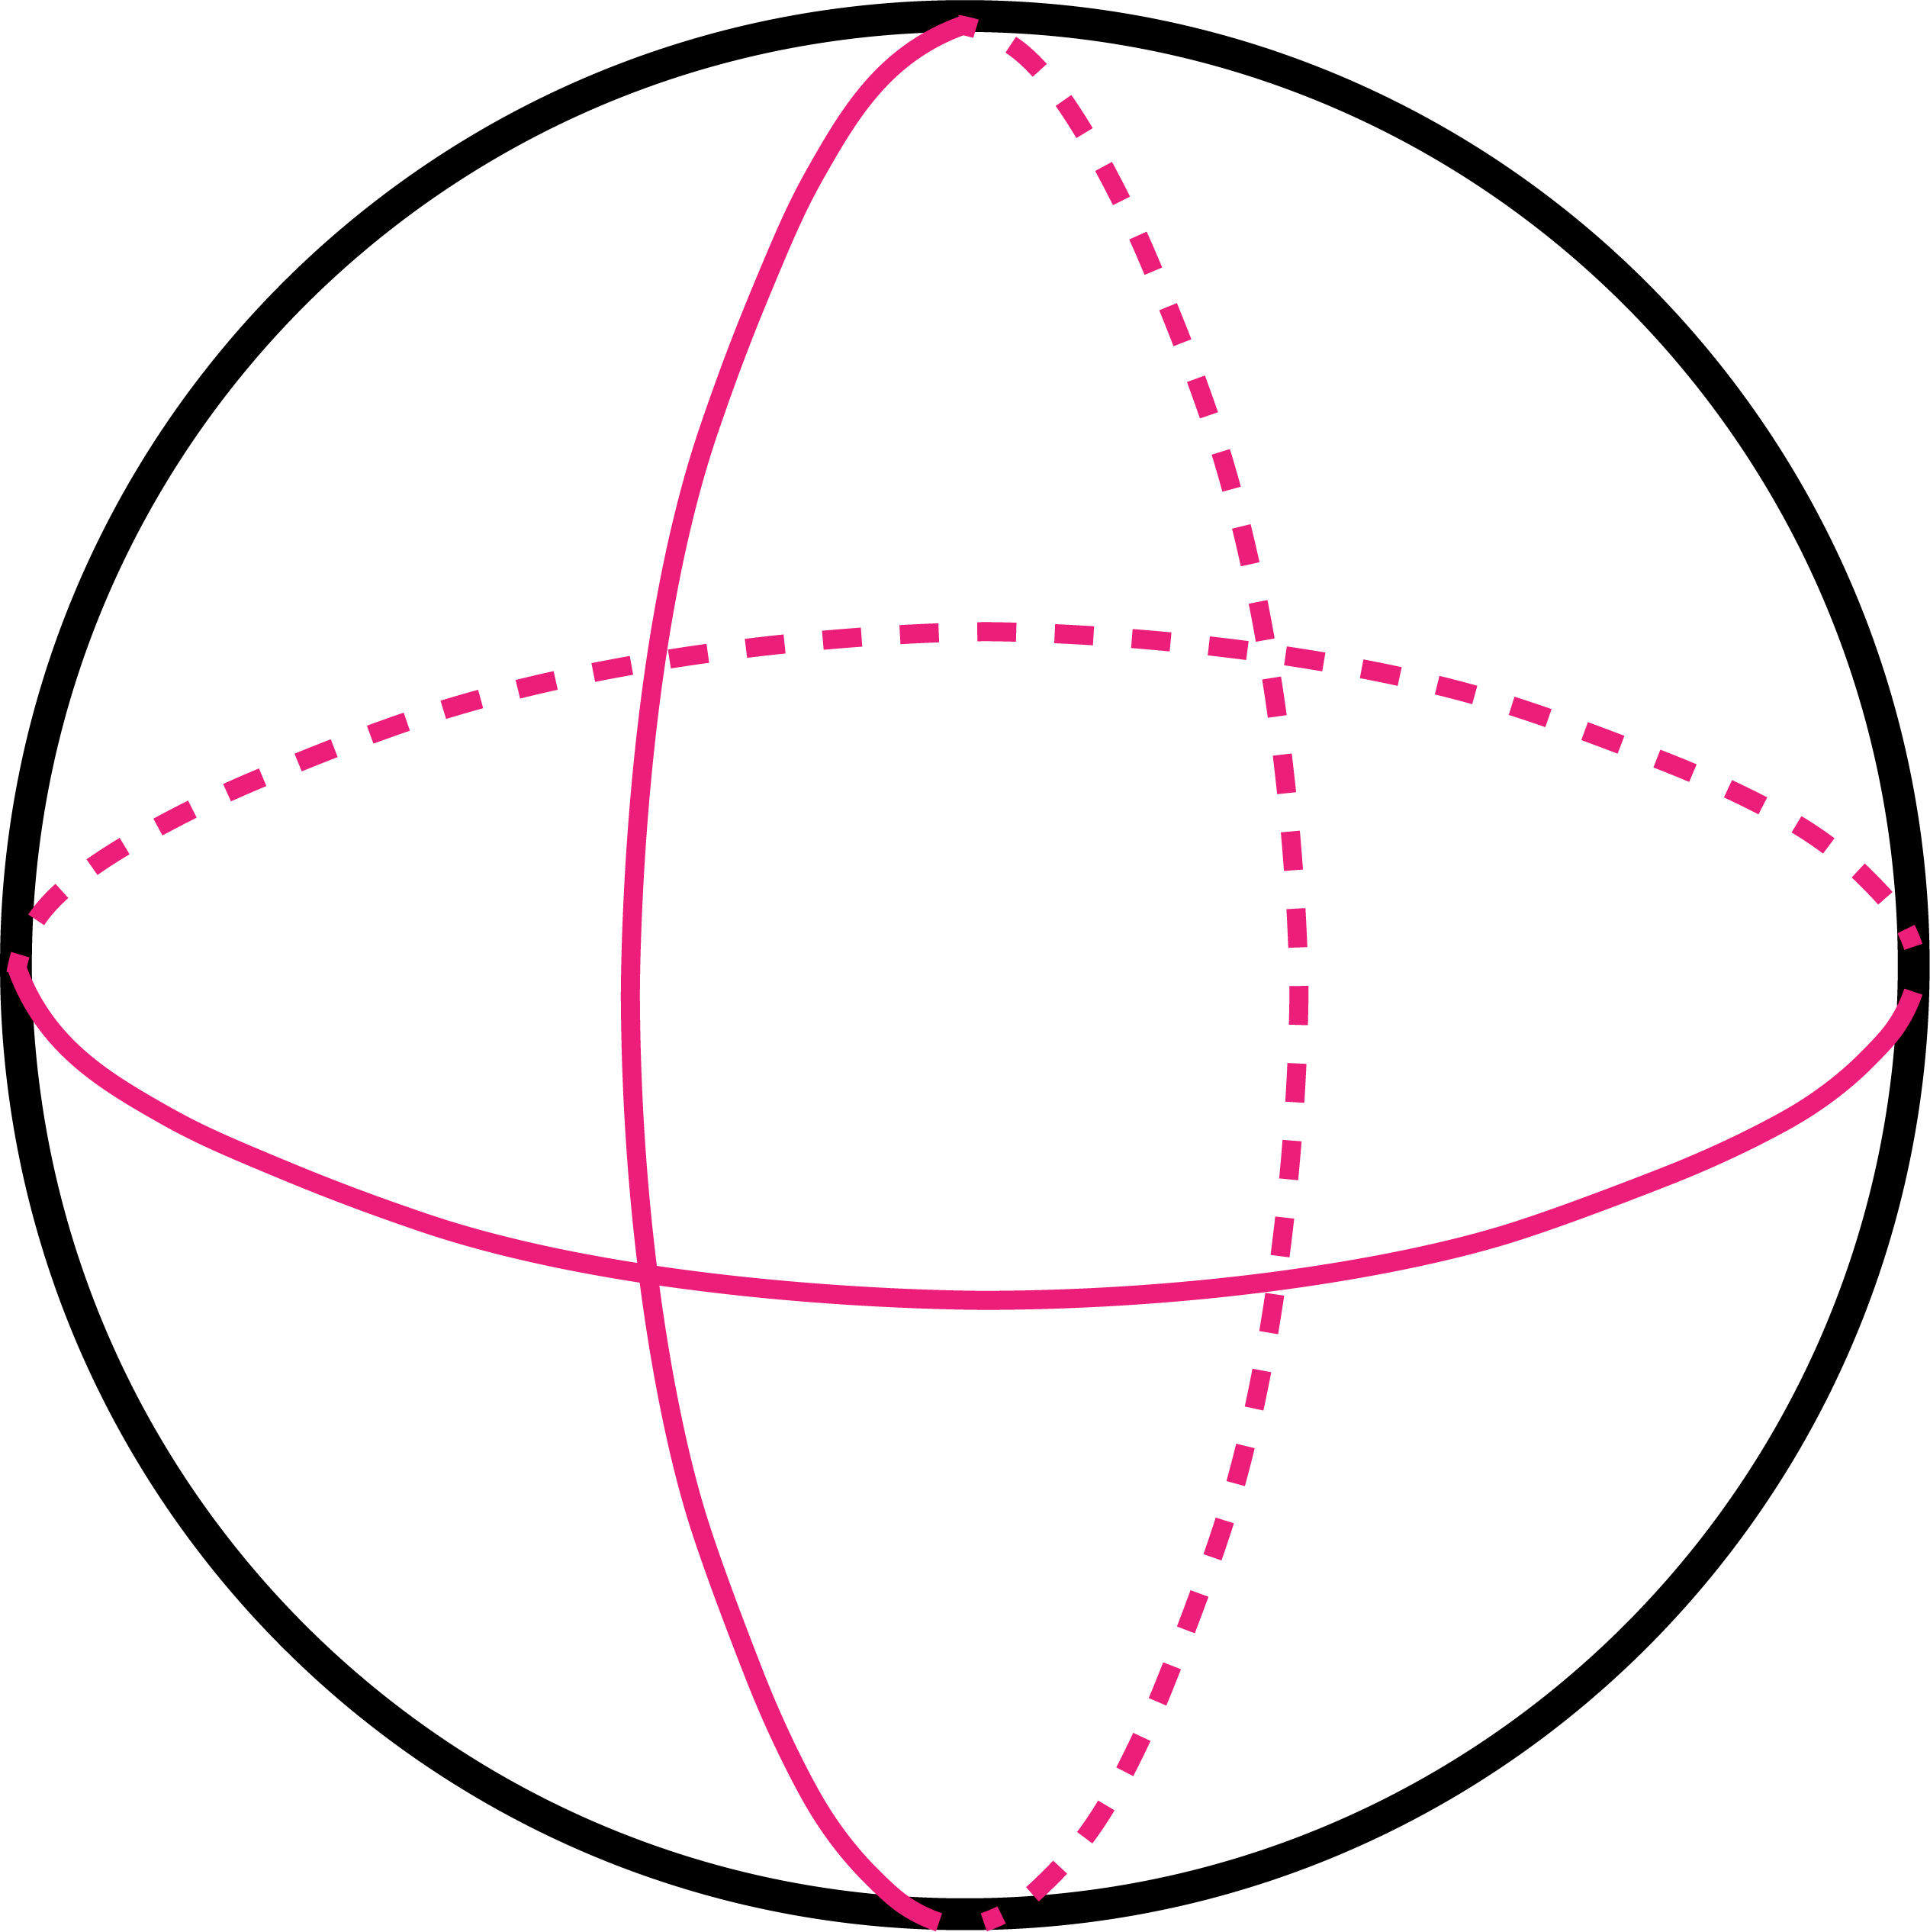
\includegraphics[width=4cm]{pics/11_4.png}
              \centering
              \caption{Геодезические кривые ---\\
              сечения, проходящие через центр}
          \end{figure}
          \begin{figure}[H]
              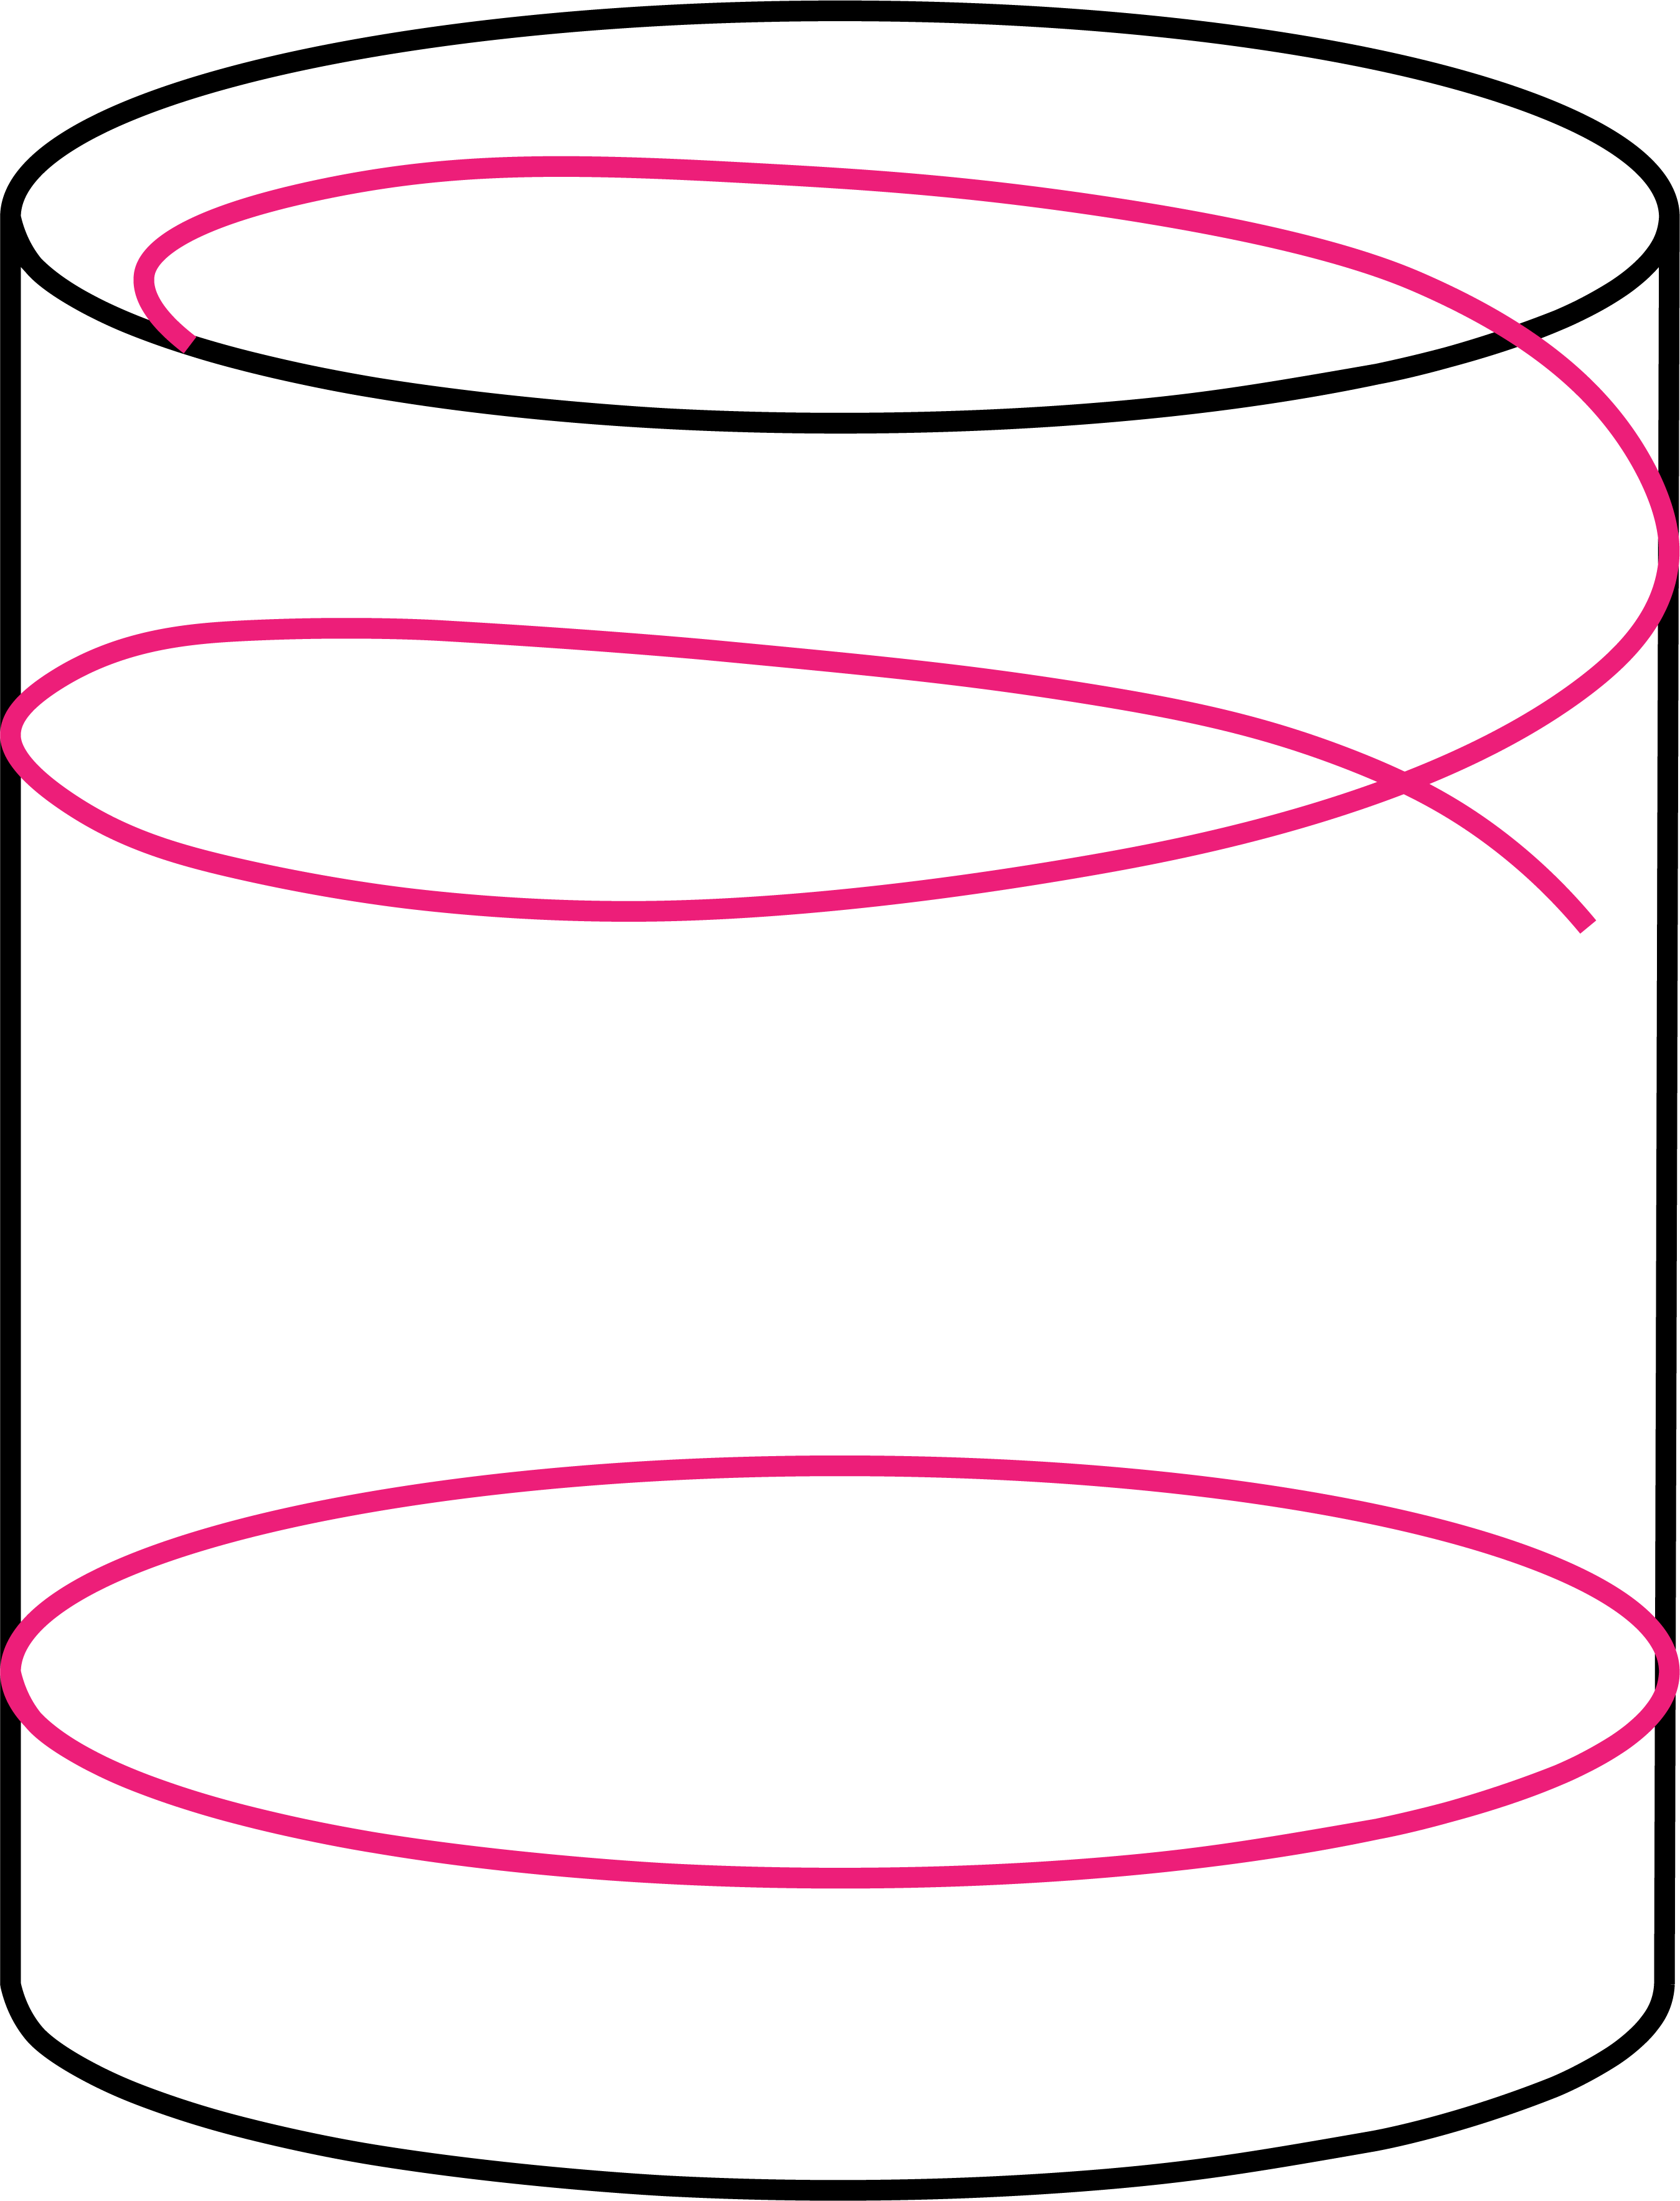
\includegraphics[width=3cm]{pics/11_5.png}
              \centering
              \caption{Геодезические кривые\\
              (спираль и окружность)}
          \end{figure}
        \end{enumerate}
    \end{utv}
\end{document}
